\documentclass{beamer}
\usetheme{Copenhagen}

\usepackage[sfdefault]{roboto} 
\usepackage[T1]{fontenc}
\usepackage{textcomp}

\newcommand\myheading[1]{%
	\par\bigskip
	{\Large\bfseries#1}\par\smallskip}

\title{Webové rozhraní pro data z IoT}
\author{Bc. Libor Michálek}

\date{Květen 2021}
\institute{VŠB – Technická Univerzita Ostrava}
\begin{document}
\begin{frame}
	\centering
    \maketitle
\end{frame}


\begin{frame}{Cíl projektu}
	\centering
	Cílem projektu bylo vytvořit webovou aplikaci, která poskytuje uživatelské rozhraní s vizualizací dat získaných z IoT zařízení a jejich analýzou. Součástí projektu je také aplikace pro automatický sběr těchto dat.
\end{frame}

\begin{frame}[t]{Použité technologie}
	\begin{columns}[t]
		\begin{column}{0.5\textwidth}
			\myheading{Hardware}
			\begin{itemize}
				\item TP-Link HS110
				\item Raspberry Pi
				\item Koncové zařízení uživatele
			\end{itemize}
		\end{column}
		\pause
		\begin{column}{0.5\textwidth}
			\myheading{Technologie}
			\begin{itemize}
				\item .NET Core \& ASP.NET Core
				\item NUnit 
				\item SQLite
				\item JavaScript \& React
				\item SASS \& BEM metodologie
				\item Libraries – ReCharts, Plotly, MaterialUI a další
			\end{itemize}
		\end{column}
	\end{columns}
\end{frame}

\begin{frame}{Struktura projektu}
	Struktura projektu byla rozdělena do \textbf{tří} částí – aplikací:
	\bigbreak
	\begin{itemize}
		\item Sběr dat
		\item Poskytování dat skrze REST API
		\item React aplikace
	\end{itemize}
\end{frame}

\begin{frame}{Struktura projektu – Schéma}
	\centering
	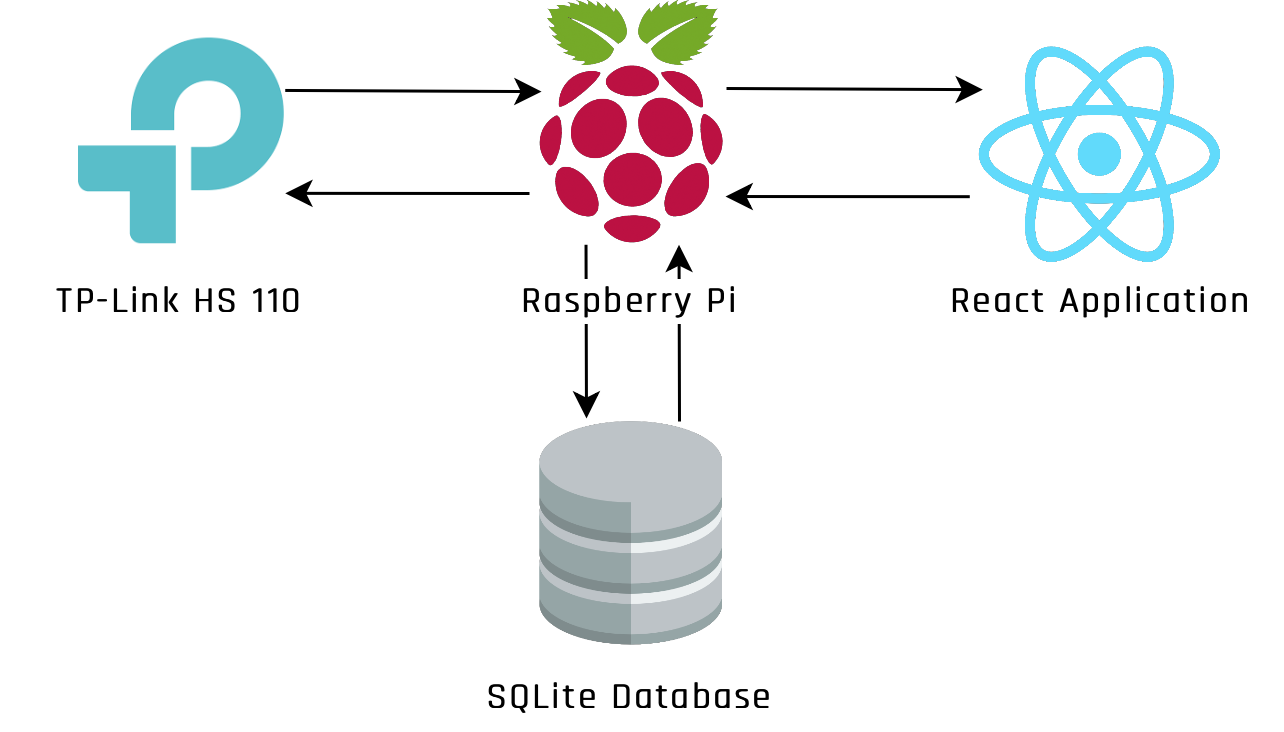
\includegraphics[scale=0.175]{AppDesign}
\end{frame}

\begin{frame}{Struktura projektu – Data Collector}
	\begin{itemize}
		\item .NET Core aplikace registrována jako systémová služba
		\item Periodicky sbírá data z chytré zásuvky a ukládá je do databáze
		\item Komunikace pomocí JSON formátu s využitím autoklíčové šifry
		\item Využívá vlastní jednoduchou ORM knihovnu
		\item Paměťová náročnost – \textasciitilde40B/záznam $\rightarrow$ ~600B/h $\rightarrow$ ~14kB/den $\rightarrow$ ~422kB/měsíc $\rightarrow$ ~4,9MB/rok
	\end{itemize}
\end{frame}

\begin{frame}{Struktura projektu – API}
	\begin{itemize}
		\item ASP.NET Core aplikace registrována jako systémová služba
		\item Poskytuje dva REST endpointy pro poskytování dat
		\item Využívá vlastní jednoduchou ORM knihovnu
		\item Paměťová náročnost – \textasciitilde74B/záznam $\rightarrow$ ~1100B/h $\rightarrow$ ~26kB/den $\rightarrow$ ~780kB/měsíc $\rightarrow$ ~9MB/rok
	\end{itemize}
\end{frame}


\begin{frame}{Struktura projektu – React Frontend}
	\begin{itemize}
		\item React aplikace využívající knihovny pro grafové vizualizace
		\item Vizualizace časových řad s naměřenými elektrickými veličinami
		\item Výpočet a vizualizace statistik – píky, průměry, mediány \& provozní časy
		\item Detekce podobností hodinových průměrů spotřeby v rámci dnů v týdnu – K-Means \& DBSCAN s vizualizací výsledků
	\end{itemize}
\end{frame}


\begin{frame}{Výsledek – Přehled se statistikami}
	\centering
	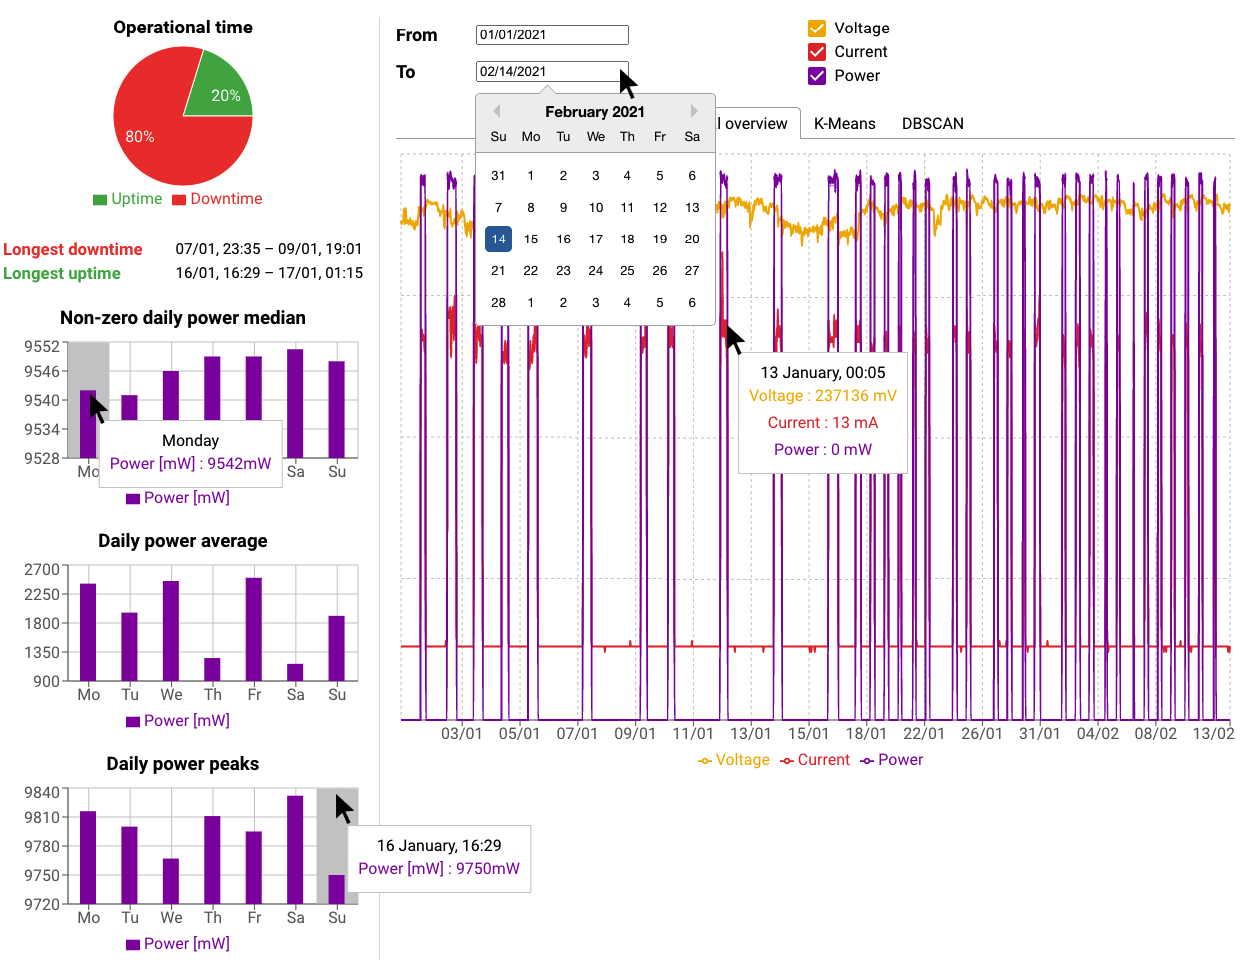
\includegraphics[scale=0.225]{React1}
\end{frame}

\begin{frame}{Výsledek – Shlukování pomocí K-Means}
	\centering
	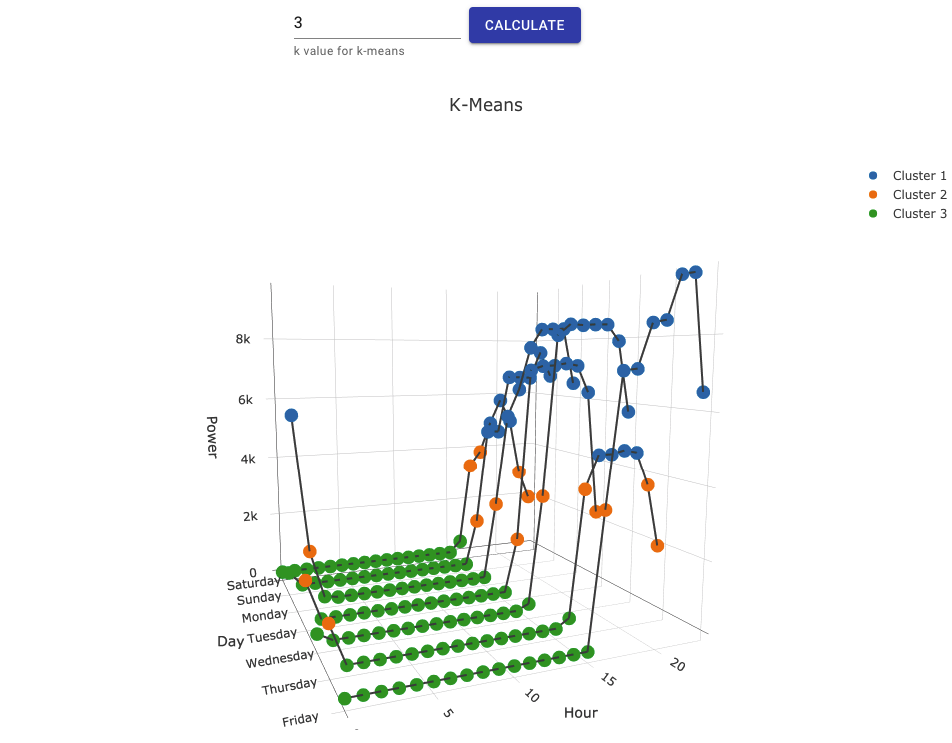
\includegraphics[scale=0.275]{React2}
\end{frame}

\begin{frame}{Výsledek – Shlukování pomocí DBSCAN}
	\centering
	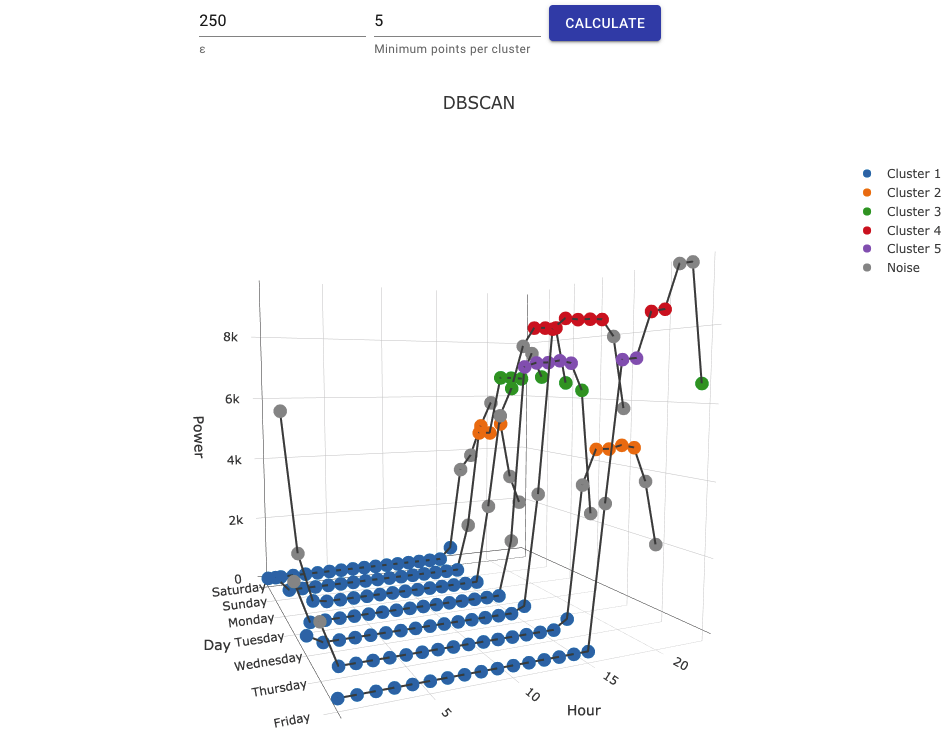
\includegraphics[scale=0.275]{React3}
\end{frame}

\begin{frame}{Výsledek – Textová reprezentace shluků}
	\centering
	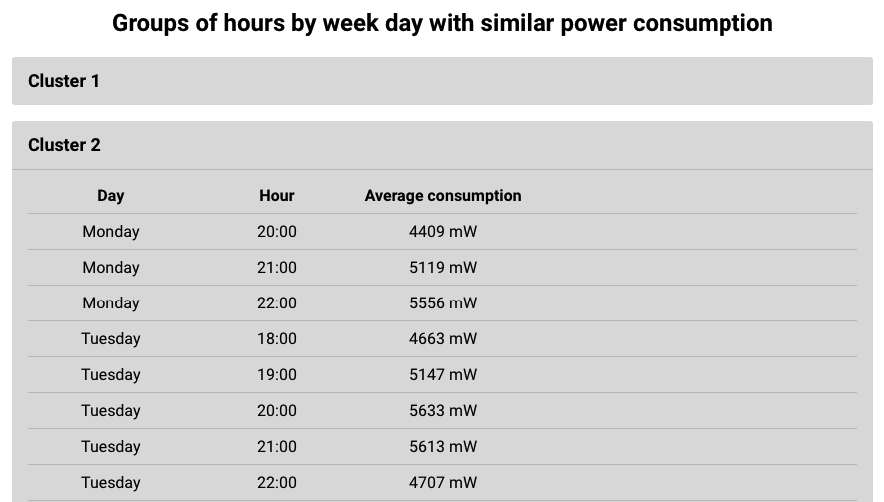
\includegraphics[scale=0.275]{React4}
\end{frame}


\begin{frame}
	\centering
	\myheading{Děkuji za Vaši pozornost}
\end{frame}



\end{document}
